\documentclass{cmc}

\begin{document}

\pagestyle{fancy}
\lhead{\textit{\textbf{Computational Motor Control, Spring 2019} \\
    Python exercise, Lab 6, GRADED}} \rhead{Student \\ Names}

\section*{Student names: \ldots (please update)}
\textit{Instructions: Update this file (or recreate a similar one,
  e.g.\ in Word) to prepare your answers to the questions. Feel free
  to add text, equations and figures as needed. Hand-written notes,
  e.g.\ for the development of equations, can also be included e.g.\
  as pictures (from your cell phone or from a scanner).
  \textbf{\corr{This lab is graded.}} and must be submitted before
  the \textbf{\corr{Deadline : 11-04-2018 Midnight}}.  \\ Please
  submit both the source file (*.doc/*.tex) and a pdf of your
  document, as well as all the used and updated Python functions in a
  single zipped file called \corr{lab6\_name1\_name2\_name3.zip} where
  name\# are the team member’s last names.  \corr{Please submit only
    one report per team!}}
\\

\textit{The file \fileref{lab\#.py} is provided to run all exercises
  in Python.
  % Each \fileref{exercise\#.py} can be run to run an exercise
  % individually.
  The list of exercises and their dependencies are shown in
  Figure~\ref{fig:files}.
  When a file is run, message logs will be printed to indicate
  information such as what is currently being run and and what is left
  to be implemented. All warning messages are only present to guide
  you in the implementation, and can be deleted whenever the
  corresponding code has been implemented correctly.}


% \textit{In this exercise, you will explore the different modeling
%   techniques that can be used to control a single joint and
%   segment. We initially start by exploring a single joint controlled
%   by a pair of antagonist spring like muscles and then extend the
%   model by adding dampers to it. These only represent the passive
%   dynamics observed in a real musculoskeletal system. To make the
%   behavior more realistic we then study more complex hill muscle model
%   in detail. }

\begin{figure}[ht]
  \centering 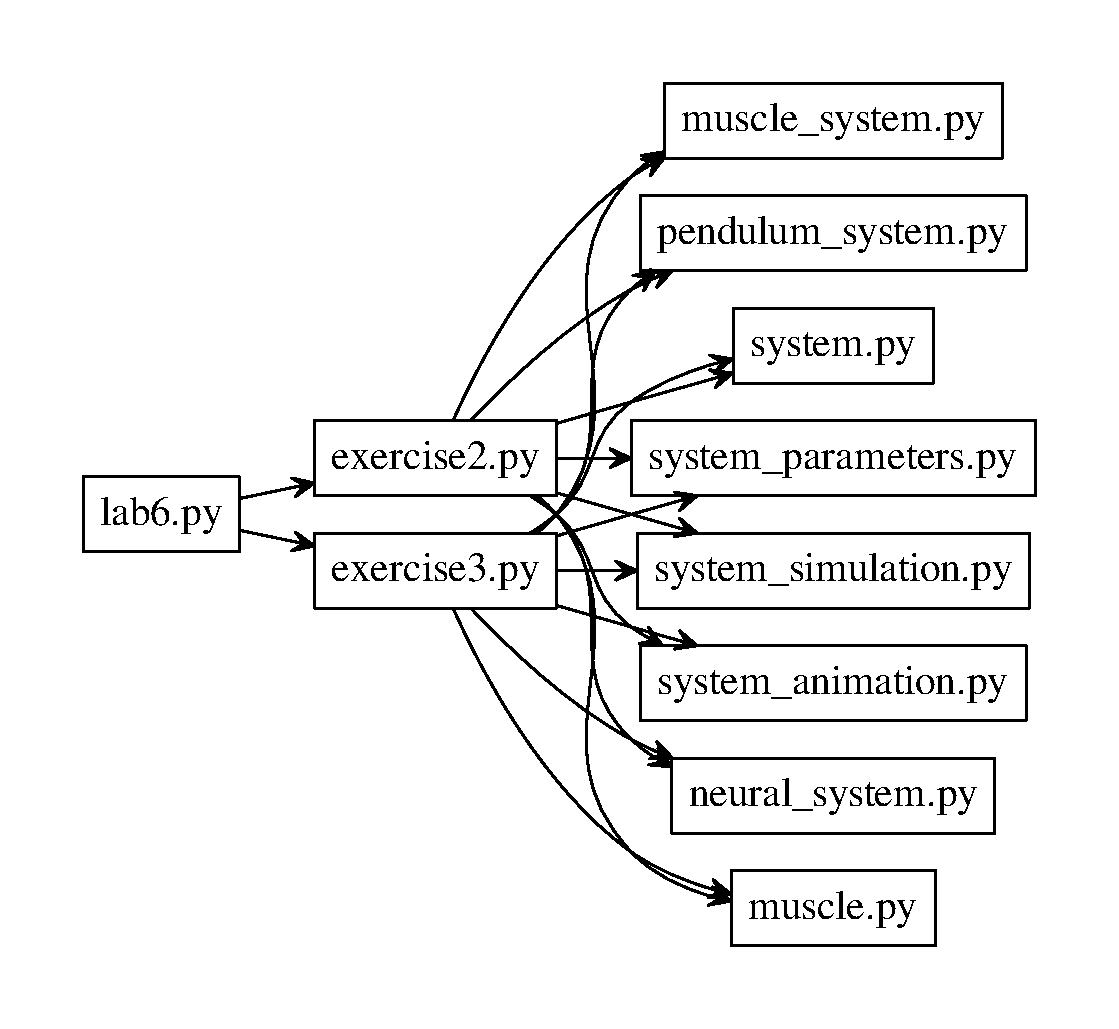
\includegraphics[width=0.5\textwidth]{figures/files}
  \caption{\label{fig:files} Exercise files dependencies. In this lab,
    you will be modifying \fileref{exercise1.py} and
    \fileref{pendulum\_system.py}}
\end{figure}

\subsection*{Files to complete the exercises}
\label{sec:intro}

\begin{itemize}
\item \fileref{lab6.py} : Main file
\item \fileref{exercise2.py} : Main file to complete exercise 2
\item \fileref{exercise3.py} : Main file to complete exercise 3
\item \fileref{system\_parameters.py} : Parameter class for Pendulum,
  Muscles and Neural Network (Create an instance and change properties
  using the instance. You do not have to modify the file)
\item \fileref{muscle.py} : Muscle class (You do not have to modify
  the file)
\item \fileref{system.py} : System class to combine different models %
  like Pendulum, Muscles, Neural Network (You do not have to modify
  the file)
\item \fileref{pendulum\_system.py} : Contains the description of
  pendulum equation and Pendulum class. You can use the file to define
  perturbations in the pendulum.
\item \fileref{muscle\_system.py} : Class to combine two muscles (You
  do not have to modify the file)
\item \fileref{neural\_system.py} : Class to describe the neural
  network (You do not have to modify the file)
\item \fileref{system\_simulation.py} : Class to initialize all the
  systems, validate and to perform integration (You do not have to
  modify the file)
\item \fileref{system\_animation.py} : Class to produce animation of
  the systems after integration (You do not have to modify the file)
\end{itemize}

\textbf{NOTE : } '\textit{You do not have to modify}' does not mean
you should not, it means it is not necessary to complete the
exercises. But, \corr{you are expected to look into each of these
  files and understand how everything works}. You are free to explore
and change any file if you feel so.

\section*{Exercise 2 : Pendulum model with Muscles}
\label{sec:question-1}

\begin{figure}[H]
  \centering 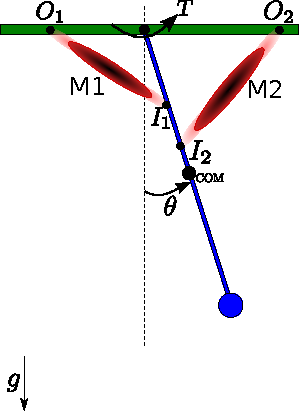
\includegraphics[scale=1.0]{figures/pendulum_muscles.pdf}
  \caption{Pendulum with Antagonist Hill Muscles}
  \label{fig:p_muscles}
\end{figure}

The system is comprised of a physical pendulum described by equation
\ref{eq:pendulum} and a pair of antagonist muscles \textbf{M1} and
\textbf{M2}. Muscle \textbf{M1} extends the pendulum ($\theta$
increases) and Muscle \textbf{M2} flexes the muscle ($\theta$
decreases).

Consider the system only for the pendulum range $\theta$ =
$[-\pi/2, \pi/2]$

\begin{equation}
  \label{eq:pendulum}
  I\ddot{\theta} = -0.5 \cdot m \cdot g \cdot L \cdot sin(\theta)
\end{equation}

Where,

\begin{itemize}
\item $I$ - Pendulum inertia about the pendulum pivot joint
  [$kg \cdot m^2$]
\item $\theta$ - Pendulum angular position with the vertical [$rad$]
\item $\ddot{\theta}$ - Pendulum angular acceleration
  [$rad \cdot s^{-2}$]
\item $m$ - Pendulum mass [$kg$]
\item $g$ - System gravity [$m \cdot s^{-2}$]
\item $L$ - Length of the pendulum [$m$]
\end{itemize}

Each muscle is modelled using the Hill-type equations that you are now
familiar with.  Muscles have two attachment points, one at the origin
and the other at the insertion point.  The origin points are denoted
by $O_{1,2}$ and the insertion points by $I_{1,2}$. The two points of
attachment dictate how the length of the muscle changes with respect
to the change in position of the pendulum.

The active and passive forces produced by the muscle are transmitted
to the pendulum via the tendons. In order to apply this force on to
the pendulum, we need to compute the moment based on the attachments
of the muscle.

Using the laws of sines and cosines, we can derive the length of
muscle and moment arm as below. The reference to the paper can be
found here
\href{https://www.ncbi.nlm.nih.gov/pmc/articles/PMC5323435}{\corr{Reference}},

\begin{eqnarray}
  \label{eq:2}
  L_1 = \sqrt[2]{a_{1}^2 + a_{2}^2 + 2 \cdot a_1 \cdot a_2 \cdot \sin(\theta)} \\
  h_1 = \frac{a_1 \cdot a_2 \cdot \cos(\theta)}{L_1}
\end{eqnarray}

Where,

\begin{itemize}
\item $L_1$ : Length of muscle 1
\item $a_1$ : Distance between muscle 1 origin and pendulum origin
  ($|O_1C|$)
\item $a_2$ : Distance between muscle 1 insertion and pendulum origin
  ($|I_1C|$)
\item $h_1$ : Moment arm of the muscle
\end{itemize}

\begin{figure}[H]
  \centering
  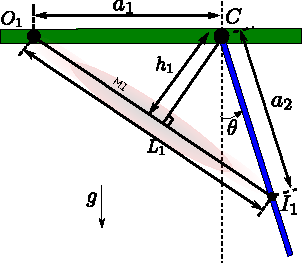
\includegraphics[scale=1]{figures/pendulum_muscles_force_length.pdf}
  \caption[force_length]{Computation of muscle length and moment arm}
  \label{fig:pendulum_muscles_force_length}
\end{figure}

Equation \ref{eq:2} can be extended to the Muscle 2 in similar
way. Thus, the final torque applied by the muscle on to the pendulum
is given by,

\begin{equation}
  \label{eq:3}
  \tau = F \cdot h
\end{equation}

Where,

\begin{itemize}
\item $\tau$ : Torque [$N \cdot m$]
\item $F$ : Muscle Tendon Force [$N$]
\item $h$ : Muscle Moment Arm [$m$]

\end{itemize}

In this exercise, the following states of the system are integrated
over time,

\begin{equation}
  \label{eq:1}
  X = \begin{bmatrix}
    \theta & \dot{\theta} & A_1 & l_{CE1} & A_2 & l_{CE2}
  \end{bmatrix}
\end{equation}

Where,

\begin{itemize}
\item $\theta$ : Angular position of the pendulum [rad]
\item $\dot{\theta}$ : Angular velocity of the pendulum [rad/s]
\item $A_1$ : Activation of muscle 1 with a range between [0, 1].  0
  corresponds to no stimulation and 1 corresponds to maximal
  stimulation.
\item $l_{CE1}$ : Length of contracticle element of muscle 1
\item $A_2$ : Activation of muscle 2 with a range between [0, 1].  0
  corresponds to no stimulation and 1 corresponds to maximal
  stimulation.
\item $l_{CE2}$ : Length of contracticle element of muscle 2
\end{itemize}

To complete this exercise you will make use of the following files,
\fileref{exercise2.py}, \fileref{system\_parameters.py},
\fileref{muscle.py}, \fileref{system.py}, \fileref{pendulum\_system.py},
\fileref{muscle\_system.py}, \fileref{system\_simulation.py} %

\label{sec:questions}

\subsection*{2a. For a given set of attachment points, compute and
  plot the muscle length and moment arm as a function of $\theta$
  between $[-\pi/4, \pi/4]$ using equations in \corr{eqn:\ref{eq:2}}
  and discuss how it influences the pendulum resting position and the
  torques muscles can apply at different joint angles. You are free to implement
this code by yourself as it does not have any other dependencies.}
\label{sec:2a}


\subsection*{2b. Using simple activation wave forms (example : sine or
  square waves) applied to muscles (use
  \fileref{system\_simulation.py::add\_muscle\_activations} method in
  \fileref{exercise2.py}), try to obtain a limit cycle behavior for
  the pendulum. Use relevant plots to prove the limit cycle behavior.
  Explain and show the activations wave forms you used. Use
  \newline \fileref{pendulum\_system.py::PendulumSystem::pendulum\_system} function to perturb the model.}
\label{sec:2c}


\subsection*{2c. Show the relationship between stimulation
  frequency and amplitude with the resulting pendulum's behavior.}
\label{sec:2e}

\newpage
\section*{Exercise 3 : Neural network driven pendulum model with
  muscles}
\label{sec:neur-netw-driv}

In this exercise, the goal is to drive the above system
\ref{fig:p_muscles} with a symmetric four-neuron oscillator
network. The network is based on Brown's half-center model with
fatigue mechanism. Here we use the leaky-integrate and fire neurons
for modelling the network. Figure \ref{fig:p_muscles_neurons} shows
the network structure and the complete system.

\begin{figure}[H]
  \centering
  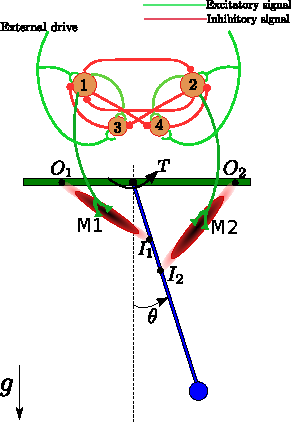
\includegraphics[scale=1.5]{figures/pendulum_muscles_neurons.pdf}
  \caption{Pendulum with Antagonist Hill Muscles Driven Half Center
    Neural Network.}
  \label{fig:p_muscles_neurons}
\end{figure}

Since each leaky-integrate and fire neuron comprises of one first
order differential equation, the states to be integrated now increases
by four(one state per neuron). The states are,


\begin{equation}
  \label{eq:1}
  X = \begin{bmatrix}
    \theta & \dot{\theta} & A_1 & l_{CE1} & A_2 & l_{CE2} & m_1 & m_2 & m_3 & m_4
  \end{bmatrix}
\end{equation}

Where,

\begin{itemize}
\item $m_1$ : Membrane potential of neuron 1
\item $m_2$ : Membrane potential of neuron 2
\item $m_3$ : Membrane potential of neuron 3
\item $m_4$ : Membrane potential of neuron 4
\end{itemize}

To complete this exercise, additionally you will have to use
\fileref{neural\_system.py} and \fileref{exercise3.py}

\subsection*{3a. Find a set of weights for the neural network that
  produces oscillations to drive the pendulum into a limit cycle
  behavior. Plot the output of the network and the phase plot of
the pendulum}
\label{sec:4a}


\subsection*{3b. As seen in the course, apply an external drive to the
  individual neurons and explain how the system is affected. Show
  plots for low [0] and high [1] external drives. To add external
  drive to the network you can use the method \\
  \fileref{system\_simulation.py::add\_external\_inputs\_to\_network} }
\label{sec:4c}


\subsection*{3c. [Open Question] What are the limitations of the half
  center model in producing alternating patterns to control the
  pendulum? What would be the effect of sensory feedback on this
  model? (No plots required)}
\label{sec:4d}


\end{document}

%%% Local Variables:
%%% mode: latex
%%% TeX-master: t
%%% End: